\documentclass[conference]{IEEEtran}
\usepackage{amsmath,amssymb,graphicx,booktabs,textcomp,url,cite}
\usepackage[T1]{fontenc}
\hyphenation{Sentinel DarkRS ExDark}
\begin{document}
\title{Can Illumination-Aware Gamma Correction Tell Shadows from Dark Surfaces? A Training-Free Redesign (TASC-v1) and a Candid Failure Analysis}
\author{\IEEEauthorblockN{[Authors to be added]}\IEEEauthorblockA{Manuscript generated from the Markdown source in \texttt{research/manuscript/}}}
\maketitle
\begin{abstract}
Satellite and aerial images are often too dark, either because the whole scene was under-exposed or because terrain and clouds cast shadows. A training-free enhancer should brighten shadows without brightening surfaces that are simply dark (water, forest, burnt ground), and it should not distort the colour relationships that analysts rely on. A previous frozen method, TASC-v0, brightened every region towards a fixed target, and a benchmark showed that this over-exposed dark scenes and damaged scene classification. We therefore designed TASC-v1: an exposure rule that is anchored on the bright end of the histogram, a local brightening step that is switched on only where there is evidence of an illumination shadow, an optional elevation-model (DEM) cue whose influence is scaled by how well it agrees with the image, no detail-boosting stage, and a single gain shared by all bands. We tested it on Landsat, Sentinel-2 with a DEM, AID, iSAID-dark, DarkRS, ExDark and a frozen classifier, with the selection criteria fixed beforehand. The redesign repaired TASC-v0's failures on synthetic low light (+3.4 dB PSNR on AID, +2.5 dB on iSAID-dark, and 15 to 31 percentage points of classification accuracy recovered) and preserved spectral angle, NDVI and band ratios exactly. It did not become a better method: it failed its own development gate on Landsat terrain data (about 9.5 dB below TASC-v0), it trails per-band gamma and Zero-DCE on every reference-based benchmark, and the DEM brought no demonstrable benefit. We conclude that the evidence supports a benchmark and failure-analysis contribution, not a new state-of-the-art enhancer.
\end{abstract}
\begin{IEEEkeywords}
low-light enhancement, gamma correction, remote sensing, shadow detection, digital elevation model, negative results.
\end{IEEEkeywords}
\section{Introduction and Motivation}
Optical remote-sensing images are routinely dark in ways that matter. A whole image may be under-exposed because of sensor settings or atmosphere, and mountainous scenes contain topographic shadows in which useful information is present but faint. Enhancement is attractive because it needs no new data. It is also risky, because enhancement that is not physically grounded can create colour casts, amplify noise, and push images away from the data distribution on which downstream models were trained.

Our earlier work introduced TASC-v0, a training-free "terrain-aware, spectrally consistent" gamma correction. A broad benchmark with corrected spectral metrics and independent statistical units exposed three weaknesses. First, TASC-v0 forced every image, and every 16-pixel block, towards the same mean brightness (0.55); on AID it reached 11.5 dB PSNR against 17.5 dB for the best simple baseline, and on iSAID-dark it scored below the unprocessed image (9.5 dB against 11.8 dB). Second, scene classification on enhanced images lost 15 to 24 percentage points of accuracy. Third, the DEM-assisted version lifted terrain shadows more strongly, but we could not show that this was physically accurate, because the shadow masks used for evaluation came from the same DEM.

This paper asks a deliberately narrow question: \emph{can a training-free enhancer be redesigned so that it (i) does not over-expose, (ii) brightens shadows but leaves naturally dark surfaces alone, (iii) trusts a DEM only as far as the image supports it, and (iv) keeps band relationships exact, and does it then generalise to independent data?} We call the redesign TASC-v1. We report what worked, what failed, and what we cannot claim. TASC-v0 remains frozen as the baseline; all new code lives in a separate package.

\section{Related Work and Research Gap}
\emph{Exposure-adaptive gamma.} Choosing a gamma from image statistics is a long-standing idea: adaptive gamma correction (AGC) and its histogram-weighted variant (AGCWD) \cite{rahman2016agc,huang2013agcwd}, and, in tone mapping, mapping a scene "key" and a high-percentile "white" level \cite{reinhard2002tonerep}. Spatially adaptive gamma for optical remote sensing has been studied (SAGC, SAMSIE) \cite{huang2018sagc,huang2022samsie}; we did not evaluate these methods, and our "2D-gamma" baseline is a different, Lee-style implementation. Retinex theory models an image as reflectance times illumination \cite{land1971retinex,jobson1997msr}, and guided filtering is a standard way to smooth such fields without halos \cite{he2013guided}.

\emph{Shadows versus dark materials.} Illumination changes alter intensity much more than chromaticity, whereas reflectance changes alter both; this underlies shadow removal in colour images \cite{finlayson2006shadows}, shadow compensation in aerial images \cite{tsai2006shadow}, and de-shadowing of satellite imagery \cite{richter2005deshadow}. Reviews note that every cue has failure cases, such as bluish shadows and dark water \cite{shahtahmassebi2013shadow}. Cloud-shadow detection uses sun--cloud geometry \cite{zhu2012fmask}.

\emph{DEM-based correction and spectral preservation.} Topographic correction (cosine, C and SCS+C) uses the Lambertian illumination angle \cite{teillet1982ccorr,soenen2005scsc,horn1981hillshading}. Haze removal by dark-object subtraction is additive, not multiplicative \cite{chavez1988dos}. A single multiplicative gain per pixel preserves band ratios by construction; that is a property, not a recovery of surface reflectance.

\emph{Learning-based methods.} Zero-DCE estimates enhancement curves without paired data \cite{guo2020zerodce}; DFFN targets low-light remote sensing with a dual-domain network \cite{yao2024dffn}. We compare against Zero-DCE only.

\emph{Research gap and what we do not claim.} Local gamma, shared gain, exposure adaptation and DEM shadow modelling are all established. The only potentially new elements here are (a) an \emph{evidence-gated} local lift that falls back to no lift when evidence is absent, and (b) a DEM trust weight estimated from image agreement. Both are testable, and Sections V and VI show that neither is demonstrated on real data.

\section{Proposed TASC-v1 Methodology}
TASC-v1 changes five things relative to TASC-v0. We introduce each idea in words first and give the equation afterwards.

\textbf{1. Exposure anchored on the bright end.} TASC-v0 set the global gamma from the \emph{mean} brightness, so a naturally dark scene was pulled up to the same level as an under-exposed one. TASC-v1 instead asks whether the brightest part of the image reaches a sensible white level. If the 95th percentile of luminance $q$ is already high, nothing is done; if it is low, a gamma that maps $q$ to a target $t$ is applied, but the result is never allowed to exceed a mean-brightness ceiling:

\begin{equation}
\gamma_0 = \min\{1,\ \max(\ln t/\ln q,\ \gamma_{\mathrm{cap}})\}, \qquad Y_1 = Y^{\gamma_0}
\end{equation}
where $\gamma_{\mathrm{cap}}$ is the smallest gamma whose output mean does not exceed the ceiling. The defaults $t = 0.55$ and ceiling $0.35$ were chosen on validation data (Section V). This is a key/white-point rule in the spirit of tone mapping, not a new idea, and a single image cannot distinguish an under-exposed scene from a dark scene without bright objects.

\textbf{2. Evidence that a dark region is a shadow.} A dark pixel is treated as a plausible shadow only when it is (a) clearly darker than its lit surround, (b) of a similar colour (log-chromaticity) to that surround, because illumination changes brightness more than colour, and (c) when a near-infrared band exists, not water-like (NDWI above zero). Each cue lies in $[0,1]$ and they are multiplied into a confidence $C$. This is a heuristic score, \emph{not} a calibrated probability:

\begin{equation}
C = D \cdot M \cdot (1 - \lambda\, W)
\end{equation}
with $D$ the darkness evidence relative to a local surround percentile, $M$ the chromatic consistency, and $W$ the NDWI-based water likelihood. The local lift is then proportional to $C$ and aims at the surround's own brightness (0.9 of it) instead of a fixed constant:

\begin{equation}
\gamma_{\mathrm{loc}} = 1 - C\,(1 - g_{\mathrm{loc}}), \qquad g_{\mathrm{loc}} = \ln(0.9\,L)/\ln Y_s
\end{equation}
so a uniformly dark scene, which has no brighter surround, receives no local lift.

\textbf{3. Confidence-weighted DEM guidance.} The DEM supplies a geometric shadow likelihood $S$ (slope, Lambertian illumination and ray-marched cast shadow, reused from TASC-v0). Because the DEM may be misregistered or paired with wrong sun angles, $S$ is averaged over three sun-angle perturbations, shifted by up to 24 pixels to best agree with the image, and trusted only according to its correlation $\rho$ with the image darkness evidence ($\rho \le 0.1$: weight 0; $\rho \ge 0.4$: weight 1). The DEM can only \emph{raise} confidence where the image is also dark, so it can never lift a pixel that the image shows to be lit:

\begin{equation}
C' = 1 - (1 - C)\,(1 - w\,S\,D)
\end{equation}
\textbf{4. No detail-enhancement stage.} TASC-v0's DCT detail step had shown no reproducible benefit; it is off by default in TASC-v1 and kept only as an ablation.

\textbf{5. Shared gain.} The final correction is one factor per pixel applied to all bands (with a soft highlight knee and a gain cap of 6 as a noise guard). Band ratios, NDVI and spectral angle to the input are therefore unchanged exactly. This does not recover surface reflectance.

TASC-v1 contains no trained component. The implementation (\texttt{research/v1/}) is deterministic, supports RGB and RGB+NIR, and has 26 unit tests covering constant and zero images, NaN inputs, sizes from 2$\times$2 upwards, clipping, spectral invariance, exposure monotonicity, shadow-versus-dark-material behaviour and DEM trust. The frozen \texttt{tasc/} package is unchanged (verified by a test against the \texttt{TASC-v0} tag).

\section{Experimental Datasets and Protocol}
\textbf{Why a protocol first.} To avoid adapting the method to the answer, the selection criteria (gates G1 to G8) were written and committed before any candidate was scored, and parameters were chosen only on development data: the AID validation split, the Landsat D2 validation split, and four Sentinel-2 development regions. Three candidates were pre-registered: exposure only (C1), exposure plus evidence-gated local lift (C2), and C2 plus DEM guidance (C3). Five amendments made during development are listed in the repository; one, an extra "gated-exposure" variant (C2b), was added after seeing a development failure and is reported only as a post-hoc row.

\textbf{Datasets.} \emph{Landsat D2}: 60 synthetic re-illuminations of 6 source crops of one scene (unit: source crop, n = 6). \emph{Sentinel-2 L2A} \cite{drusch2012s2} \emph{with Copernicus DEM}: 6 regions, 4 development and 2 held out in earlier work (unit: region, n = 6); shadow and dark-material masks derive from the same DEM and are \emph{proxies}. \emph{AID} \cite{xia2017aid}: 210 test source images under three synthetic degradations (uniform, non-uniform, severe). \emph{iSAID-dark}: 46 parent images (synthetically darkened). \emph{DarkRS} (86 images) and \emph{ExDark} \cite{loh2019exdark} (400 images): real low light, no reference, NIQE \cite{mittal2013niqe}, BRISQUE \cite{mittal2012brisque}, entropy and similar no-reference measures only. Full-reference perceptual distance is LPIPS \cite{zhang2018lpips}. \emph{Classification}: a frozen ResNet-50 \cite{he2016resnet} with a logistic-regression head trained once on 900 clean, disjoint AID images, applied to the 210 test images after degradation and enhancement.

\textbf{Reuse of Phase 3 results.} Baseline rows (Zero-DCE, CLAHE \cite{zuiderveld1994clahe}, global gamma, and so on) come from the earlier stores, which use identical inputs. The recomputed TASC-v0 and unprocessed rows matched the stored values to $0.0$ on D2, Sentinel-2 and AID. AID, iSAID-dark, D2 and Sentinel-2 test and held-out splits and the classifier test images are \emph{previously examined in Phase 3}; they were not used for tuning in Phase 4, but they are not "newly unseen". Fresh independent scenes were not obtained.

\textbf{Statistics.} Paired differences with 95 \% bootstrap intervals (10 000 resamples) over the independent units; Wilcoxon signed-rank tests with Holm correction \cite{holm1979} within each dataset-by-metric family; exact McNemar tests on paired classifier predictions. With six units the smallest attainable Wilcoxon p-value is 0.031, so no D2 or Sentinel-2 comparison can be significant after correction.

\section{Quantitative and Qualitative Results}
\subsection{What the development stage showed (before any test data)}
The development gate was failed. On AID validation, C2 improved on TASC-v0 by 4.5 dB, but on Landsat D2 validation every candidate was about 6.5 dB \emph{below} TASC-v0. The diagnosis was a conflict between two development sets: clean AID images are fairly dark, so an exposure ceiling of 0.35 protects them, whereas the Landsat crops are bright (clean mean luminance about 0.5), so the same ceiling stops the output far too early. A single-image exposure rule could not satisfy both. A smooth evidence gate on exposure (C2b) narrowed the D2 gap to 1 to 2 dB but then lifted clean AID images by more than the permitted 0.02 in luminance. By the pre-registered rule no candidate was selected. The frozen candidates were nevertheless evaluated on the final datasets, as a diagnostic.

\subsection{Synthetic low light: AID and iSAID-dark}
Table~\ref{tab:aid} and Fig.~\ref{fig:delta} show the central result. Relative to TASC-v0, TASC-v1 (C2) is better by 3.35 dB PSNR on AID (95 \% CI 2.74 to 3.99, $p_{Holm}$ < $10^{-1}$5), by 0.16 SSIM, and by 0.18 LPIPS, and it exceeds the unprocessed input by 4.5 dB. On iSAID-dark it removes the below-input failure (11.96 dB against 11.78 dB for the unprocessed image; the difference of +0.19 dB, CI $-$0.36 to 0.69, is not distinguishable from zero) and improves on TASC-v0 by 2.45 dB (CI 1.86 to 3.00). It does not reach the strongest baselines: per-band global gamma is 2.64 dB better on AID and 2.44 dB better on iSAID-dark, and Zero-DCE is 1.59 dB and 1.42 dB better.

\begin{table}[t]
\caption{AID test (210 source images; three degradations averaged) and iSAID-dark (46 parent images). Higher PSNR and SSIM, lower LPIPS are better. Per-band methods change band ratios.}
\label{tab:aid}
\centering\scriptsize
\setlength{\tabcolsep}{2.5pt}
\resizebox{\columnwidth}{!}{%
\begin{tabular}{lccccc}
\toprule
Method & AID PSNR & AID SSIM & AID LPIPS & iSAID PSNR & iSAID SSIM \\
\midrule
Unprocessed input & 10.32 & 0.256 & 0.594 & 11.78 & 0.201 \\
TASC-v0 (frozen) & 11.51 & 0.211 & 0.763 & 9.51 & 0.098 \\
TASC-v0 without global exposure & 15.56 & 0.317 & 0.651 & 10.98 & 0.120 \\
TASC-v1 C1 (exposure only) & 14.82 & 0.374 & 0.581 & 11.96 & 0.162 \\
\textbf{TASC-v1 C2} & 14.86 & 0.374 & 0.584 & 11.96 & 0.161 \\
TASC-v1 C2b (post hoc) & 15.36 & 0.347 & 0.606 & 11.04 & 0.137 \\
Global gamma (shared gain) & 15.66 & 0.308 & 0.659 & 11.13 & 0.112 \\
CLAHE & 13.66 & 0.376 & 0.594 & 12.96 & 0.176 \\
Zero-DCE & 16.46 & 0.420 & 0.575 & 13.38 & 0.185 \\
Per-band global gamma & \textbf{17.51} & \textbf{0.490} & \textbf{0.555} & \textbf{14.40} & \textbf{0.208} \\
\bottomrule
\end{tabular}}
\end{table}
\begin{figure}[t]
\centering
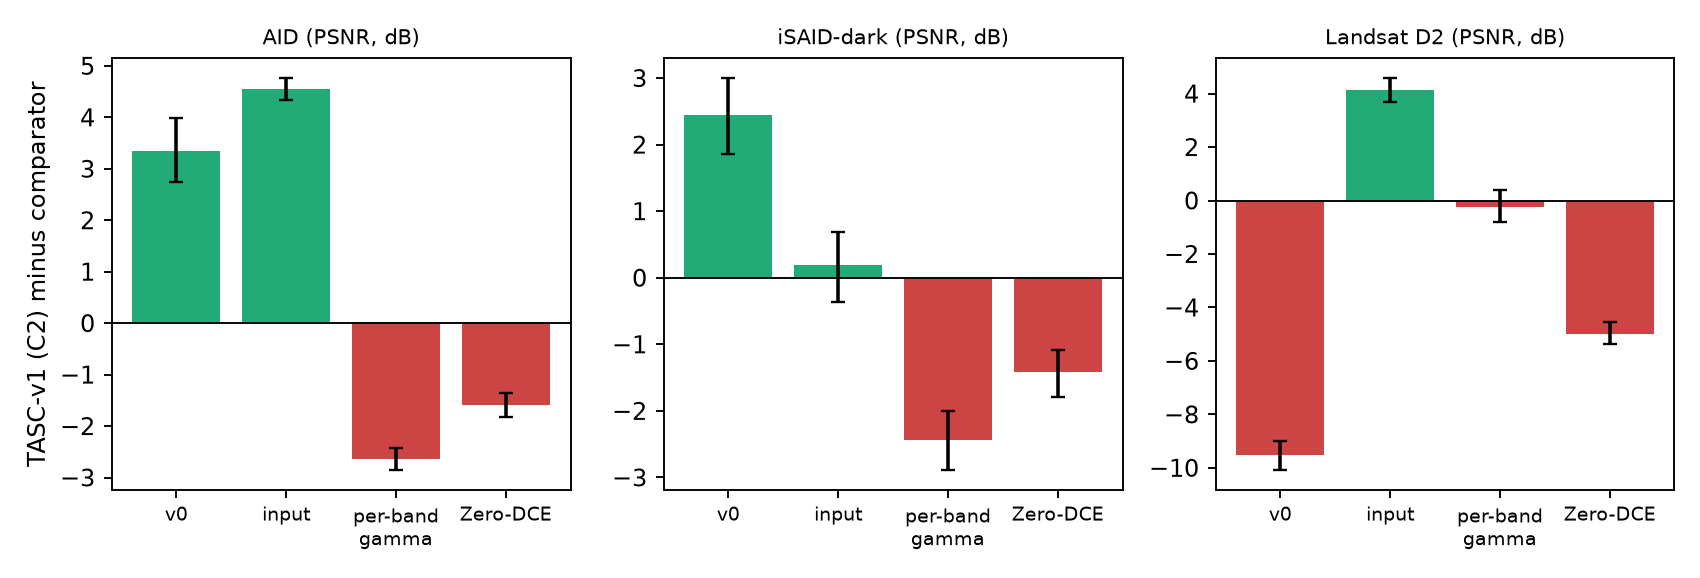
\includegraphics[width=0.95\columnwidth]{../figures/phase4/fig_delta_psnr.png}
\caption{TASC-v1 (C2) minus each comparator in PSNR, with 95 \% bootstrap intervals over independent units. Green: C2 better; red: worse. The sizeable gain over TASC-v0 on AID and iSAID-dark contrasts with a large loss on Landsat D2.}
\label{fig:delta}
\end{figure}
Part of the per-band advantage is an artefact of the benchmark. The AID degradation is a per-channel power law, which also distorts colour; a method that preserves band ratios cannot undo that, whereas per-band gamma can. A luminance-only check on the validation split still favoured global gamma over C2 (18.66 against 16.54 dB), so the gap is not only about colour. Performance by degradation is consistent: C2 gains most on the uniform case (16.74 dB, against 12.50 for TASC-v0 and 21.10 for per-band gamma) and the severe case remains hard for every method (11.31 dB for C2).

Fig.~\ref{fig:qaid} shows why TASC-v0 failed: it turns dark inputs into garish, over-saturated images, whereas TASC-v1 stays natural but slightly dark. The middle row is a failure of TASC-v1, which is visibly darker and lower in contrast than the reference.

\begin{figure}[t]
\centering
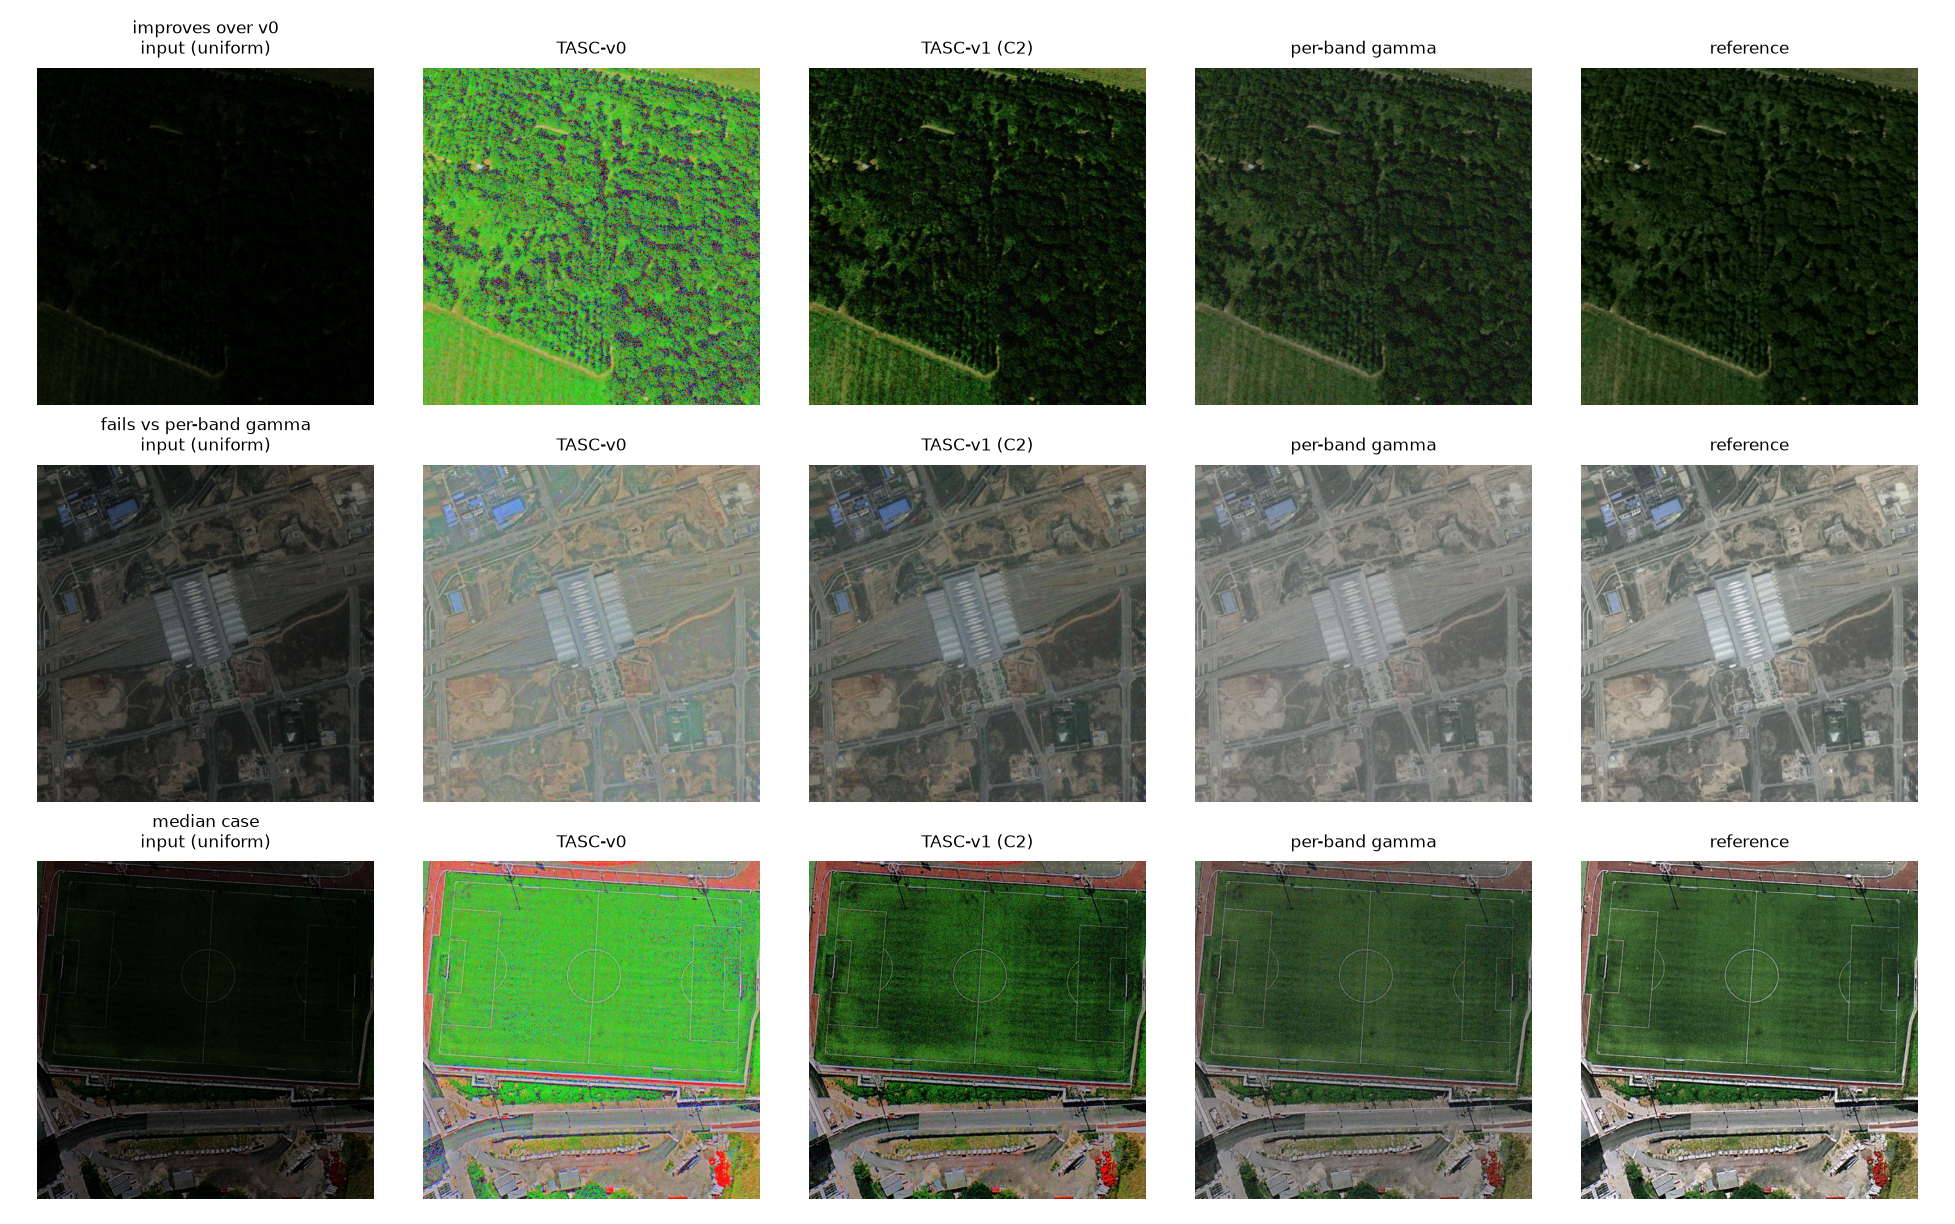
\includegraphics[width=1.0\columnwidth]{../figures/phase4/fig_qual_aid.png}
\caption{AID examples (uniform degradation). Rows: largest improvement over TASC-v0, largest deficit to per-band gamma, and a median case. Columns: degraded input, TASC-v0, TASC-v1 (C2), per-band gamma, clean reference.}
\label{fig:qaid}
\end{figure}
\subsection{Downstream classification}
Table~\ref{tab:cls} repeats the Phase 3 probe with the same frozen network and head. TASC-v0 lost 14.8 to 23.8 percentage points against the unprocessed input; TASC-v1 removes that loss. Against TASC-v0, accuracy is higher by 15.2, 19.0 and 30.5 points (non-uniform, uniform, severe; all $p_{Holm}$ < 0.001). Against the unprocessed input, the differences are $-$1.0, 0.0 and +6.7 points; only the severe case looks like a gain (McNemar p = 0.009), and it does not survive Holm correction across the family ($p_{Holm}$ = 0.25). The honest summary is "preserves, not improves". Zero-DCE is higher in the uniform case (0.857 against 0.829).

\begin{table}[t]
\caption{Classification accuracy of a frozen ResNet-50 + logistic head on 210 test images after degradation and enhancement.}
\label{tab:cls}
\centering\scriptsize
\setlength{\tabcolsep}{2.5pt}
\resizebox{\columnwidth}{!}{%
\begin{tabular}{lccc}
\toprule
Method & Uniform & Non-uniform & Severe \\
\midrule
Clean reference & 0.881 & 0.881 & 0.881 \\
Unprocessed input & 0.838 & 0.857 & 0.581 \\
TASC-v0 & 0.638 & 0.705 & 0.343 \\
TASC-v1 C1 & 0.833 & 0.871 & 0.648 \\
\textbf{TASC-v1 C2} & 0.829 & 0.857 & 0.648 \\
Per-band global gamma & 0.824 & 0.852 & 0.610 \\
Zero-DCE & 0.857 & 0.833 & 0.624 \\
\bottomrule
\end{tabular}}
\end{table}
\subsection{Real low light without references: DarkRS and ExDark}
Without references we report no-reference measures only, and they are weak evidence. On DarkRS (86 images) TASC-v1 raises entropy (6.83 against 6.48 unprocessed and 6.06 for TASC-v0) while NIQE is statistically unchanged from TASC-v0 ($-0.06$, CI $-$0.15 to 0.03). On ExDark (400 images) entropy rises (6.36 against 5.80 unprocessed) and NIQE improves over the unprocessed input ($-$0.36, CI $-$0.53 to $-$0.19), but TASC-v1 is slightly worse than TASC-v0 on NIQE (+0.20, $p_{Holm}$ = 0.04). Zero-DCE gives higher entropy on both sets. Such scores do not show that images look better to an analyst.

\subsection{Terrain shadows: Landsat D2}
Table~\ref{tab:d2} is the clearest negative result. On D2 the standard TASC-v1 configuration reaches 11.90 dB, against 21.65 dB for DEM-assisted TASC-v0 and 19.22 dB for simple global gamma; the 9.75 dB loss (CI $-$10.30 to $-$9.22, six crops of one Landsat scene) is large, but no comparison is significant after Holm correction because n = 6. The post-hoc C2b variant, which applies exposure only when there is evidence of under-exposure, scores 20.23 dB, nearer to but still below TASC-v0. The local stage and the DEM add almost nothing: C3 is only 0.07 dB above C2 (CI 0.056 to 0.081), and without the exposure stage C3 falls to 8.04 dB, close to the unprocessed input (7.78 dB).

\begin{table}[t]
\caption{Landsat D2 test (60 variants of 6 source crops; means over crops). MAE is measured in terrain-shadow pixels.}
\label{tab:d2}
\centering\scriptsize
\setlength{\tabcolsep}{2.5pt}
\resizebox{\columnwidth}{!}{%
\begin{tabular}{lcccc}
\toprule
Method & PSNR & SSIM & LPIPS & MAE shadow \\
\midrule
Unprocessed input & 7.78 & 0.361 & 0.536 & 0.468 \\
TASC-v0 (DEM, frozen) & \textbf{21.65} & 0.644 & 0.202 & \textbf{0.130} \\
TASC-v1 C1 & 11.65 & 0.439 & 0.462 & 0.382 \\
TASC-v1 C2 & 11.90 & 0.444 & 0.450 & 0.355 \\
TASC-v1 C3 (DEM) & 11.97 & 0.445 & 0.446 & 0.347 \\
TASC-v1 C2b (post hoc) & 20.23 & 0.641 & 0.248 & 0.212 \\
Global gamma & 19.22 & 0.598 & 0.270 & 0.224 \\
Zero-DCE & 16.89 & 0.490 & 0.481 & 0.297 \\
\bottomrule
\end{tabular}}
\end{table}
\begin{figure}[t]
\centering
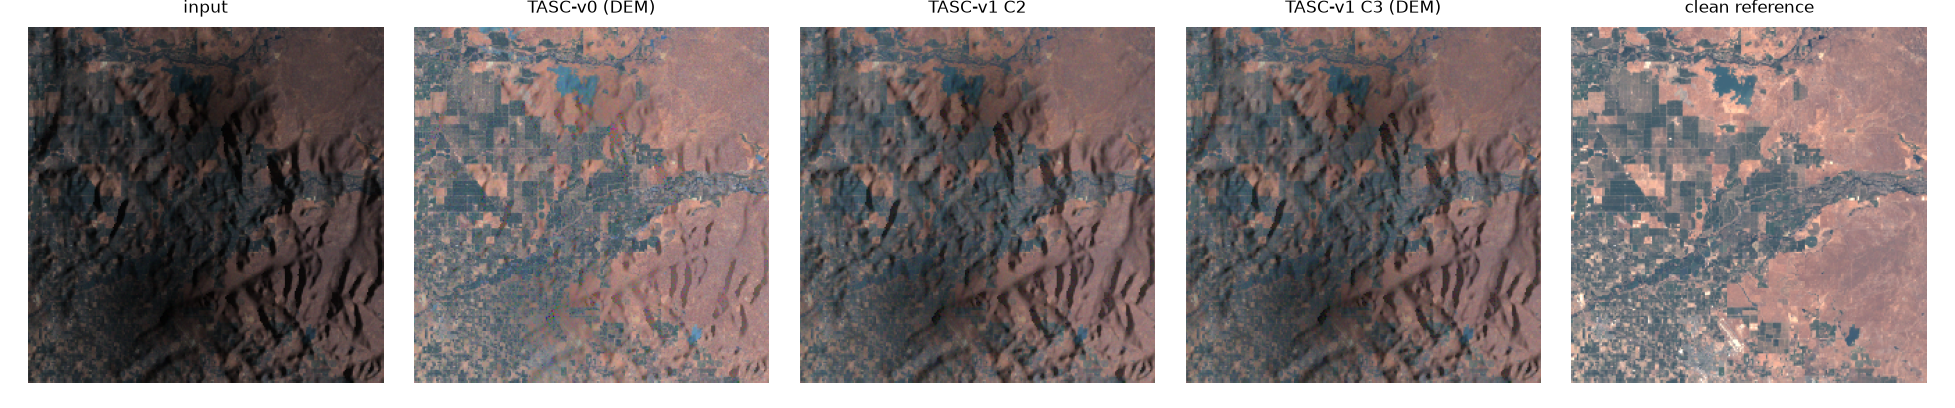
\includegraphics[width=1.0\columnwidth]{../figures/phase4/fig_qual_d2.png}
\caption{Landsat D2 example. TASC-v0 recovers most of the scene; TASC-v1 leaves much of the terrain shadow.}
\label{fig:qd2}
\end{figure}
\subsection{Terrain shadows on real data: Sentinel-2 with a DEM}
Sentinel-2 has no ground-truth illumination, so this analysis is \textbf{exploratory and proxy-based}: shadow and lit masks come from the same DEM that C3 may use, and the lit/dark material classes come from spectral indices that are independent of the DEM. Table~\ref{tab:s2} gives region means (n = 6). Spectral angle to the input, NDVI error and band-ratio deviation are exactly 0 for every shared-gain method, as expected by construction; the per-band variants change spectra (SAM 7.1$^{\circ}$ for the per-band TASC-v1 variant and 9.2$^{\circ}$ for per-band global gamma).

TASC-v1 lifts shadow pixels by 0.053, against 0.164 for TASC-v0 and 0.198 for DEM-assisted TASC-v0. It also lifts naturally dark, lit pixels less (0.024 against 0.080, CI of difference $-$0.080 to $-$0.036). This is \emph{not} evidence of better discrimination, because the ratio of dark-surface lift to shadow lift is similar (0.45 for TASC-v1 against 0.49 for TASC-v0): TASC-v1 simply enhances less everywhere. The DEM-guided variant lifts shadows by 0.004 more than image-only (CI 0.001 to 0.007), but its material-matched equalisation score is \emph{lower} ($-$0.038 against +0.043; CI of difference $-$0.162 to $-$0.009), and the DEM trust weight matters: without it the equalisation score falls to $-$0.181. A wrong DEM or a DEM shifted by 1 km behaves like image-only (0.054 and 0.055 lift). So the trust mechanism does what it was designed to do, which is to prevent harm, but no benefit from a correct DEM is demonstrated.

\begin{table}[t]
\caption{Sentinel-2 + Copernicus DEM, region means (n = 6). Lift = mean luminance gain; equalisation = reduction of shadow/lit brightness gap in vegetation (proxy).}
\label{tab:s2}
\centering\scriptsize
\setlength{\tabcolsep}{2.5pt}
\resizebox{\columnwidth}{!}{%
\begin{tabular}{lcccc}
\toprule
Method & Lift shadow & Lift dark-lit & Equalisation & SAM to input ($^{\circ}$) \\
\midrule
TASC-v0 & 0.164 & 0.080 & 0.026 & 0.00 \\
TASC-v0 + DEM & 0.198 & 0.059 & $-$0.136 & 0.00 \\
TASC-v1 C2 & 0.053 & 0.024 & 0.043 & 0.00 \\
TASC-v1 C3 (DEM) & 0.057 & 0.025 & $-$0.038 & 0.00 \\
C3 with wrong DEM & 0.054 & 0.025 & 0.056 & 0.00 \\
C3 without trust weight & 0.067 & 0.029 & $-$0.181 & 0.00 \\
C2 per band & 0.076 & 0.049 & 0.404 & 7.13 \\
Per-band global gamma & 0.111 & 0.051 & 0.565 & 9.22 \\
Zero-DCE & 0.121 & 0.067 & 0.041 & 2.20 \\
\bottomrule
\end{tabular}}
\end{table}
\begin{figure}[t]
\centering
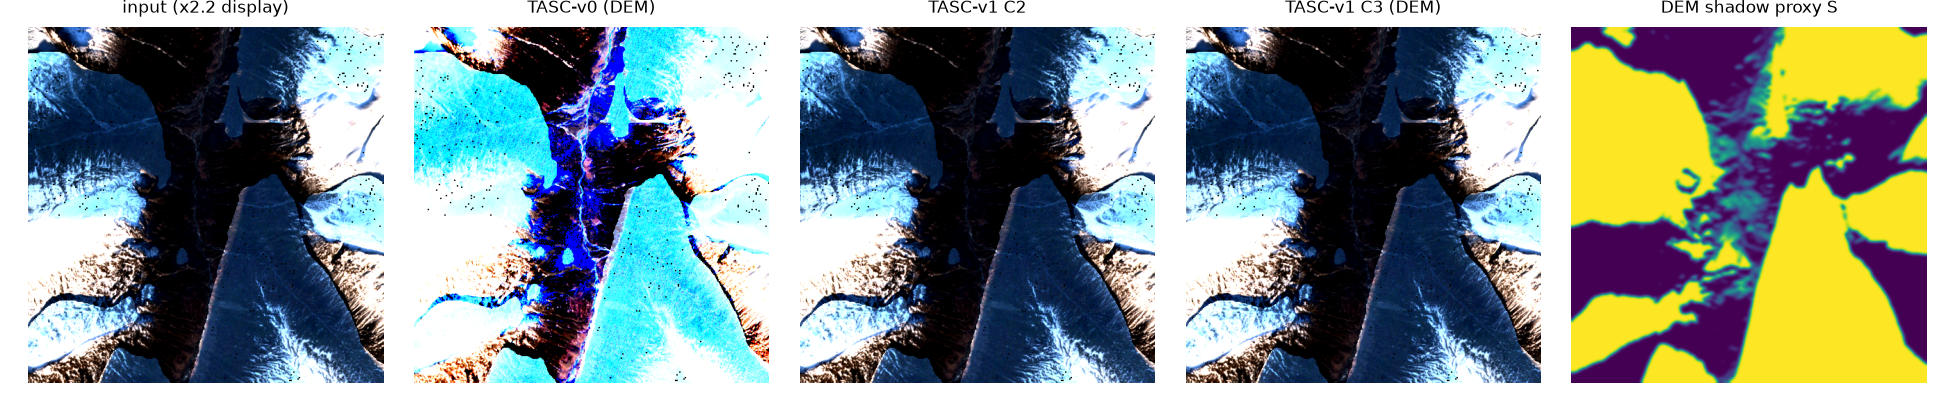
\includegraphics[width=1.0\columnwidth]{../figures/phase4/fig_qual_s2.png}
\caption{A shadowed glacier tile (held-out region), shown with display gain 2.2. TASC-v0 with DEM floods shadowed snow and ice with saturated cyan--blue (over-enhancement); TASC-v1 changes little (under-enhancement). Right: the DEM shadow proxy.}
\label{fig:qs2}
\end{figure}
\subsection{Efficiency}
Table~\ref{tab:eff} gives CPU timings (one 1024 $\times$ 1024 image, four threads, one fresh process per method; peak memory is the process high-water mark). TASC-v1 is about five times slower than TASC-v0 (the percentile filter, chromatic consistency and guided filter dominate), and the DEM-assisted version about 3.4 times slower than DEM-assisted TASC-v0 because of the sun-angle ensemble. It is still more than 40 times faster than Zero-DCE on CPU. No GPU measurements were made. An earlier Phase 3 memory column was invalid (identical for every method) and is replaced here.

\begin{table}[t]
\caption{CPU runtime and peak memory, 1024 $\times$ 1024 image.}
\label{tab:eff}
\centering\scriptsize
\setlength{\tabcolsep}{2.5pt}
\resizebox{\columnwidth}{!}{%
\begin{tabular}{lcc}
\toprule
Method & ms per megapixel & Peak memory (MB) \\
\midrule
Per-band global gamma & 22 & 166 \\
CLAHE & 14 & 167 \\
TASC-v0 & 109 & 218 \\
TASC-v0 + DEM & 218 & 247 \\
TASC-v1 C1 & 115 & 206 \\
TASC-v1 C2 & 550 & 311 \\
TASC-v1 C3 (DEM) & 743 & 311 \\
Zero-DCE & 31 788 & 1 749 \\
\bottomrule
\end{tabular}}
\end{table}
\section{Ablation Studies}
The ablations ask which ingredient produced the gains. They are summarised in Table~\ref{tab:abl}.

\begin{table}[t]
\caption{Ablations of TASC-v1 C2 (test data). PSNR in dB. A dash means the variant was not run on that dataset.}
\label{tab:abl}
\centering\scriptsize
\setlength{\tabcolsep}{2.5pt}
\resizebox{\columnwidth}{!}{%
\begin{tabular}{lccc}
\toprule
Variant & AID PSNR & iSAID PSNR & D2 PSNR \\
\midrule
C2 (full image-only) & 14.86 & 11.96 & 11.90 \\
without exposure stage & 10.45 & 11.81 & 8.04 (C3) \\
v0-style fixed exposure (mean to 0.55) & 15.76 & 11.12 & --- \\
without chromatic-consistency cue & 14.87 & 11.95 & --- \\
with DCT detail & 14.88 & 11.93 & 11.92 (C3) \\
per-band instead of shared gain & 16.29 & 13.64 & 10.74 (C3) \\
local stage removed (C1) & 14.82 & 11.96 & 11.65 \\
\bottomrule
\end{tabular}}
\end{table}
\emph{Exposure is the dominant component.} Removing it drops AID by 4.4 dB. Replacing the adaptive rule by v0's fixed mean target gives a \emph{higher} AID score (15.76 dB), but a lower iSAID-dark score (11.12 against 11.96) and, on the shadow and adequate-exposure development tests, it over-brightens correctly exposed images. The adaptive rule's benefit is therefore protective, not a universal accuracy gain.

\emph{The local stage and the chromatic cue do almost nothing on these benchmarks.} The local stage adds 0.04 dB on AID and 0.24 dB on D2. In the synthetic shadow development test, where shadow truth is known, it added 4.2 dB inside shadows (CI 3.6 to 4.9) and the chromatic cue lowered the lift of unshadowed dark pixels by about a third; that is the only direct evidence for the shadow-discrimination idea, and it is synthetic.

\emph{The DCT detail stage adds nothing} ($\pm$0.03 dB), supporting its removal. \emph{Per-band gamma scores higher} on AID and iSAID-dark, but it alters spectra (spectral angle 7 to 9$^{\circ}$) and, on D2, scores lower.

\section{Statistical Analysis}
Table Table~\ref{tab:stat} summarises the principal paired contrasts. Units: AID source image (n = 210), iSAID parent image (n = 46), D2 source crop (n = 6), Sentinel-2 region (n = 6), DarkRS and ExDark images (n = 86 and 400; image dependence within a source is not modelled), classification paired predictions (n = 210). Holm correction is applied within each dataset-by-metric family (about 20 comparators).

\begin{table}[t]
\caption{Principal paired contrasts, TASC-v1 C2 minus comparator (PSNR in dB). Intervals are 95 \% bootstrap intervals over the units.}
\label{tab:stat}
\centering\scriptsize
\setlength{\tabcolsep}{2.5pt}
\resizebox{\columnwidth}{!}{%
\begin{tabular}{lcccc}
\toprule
Dataset (unit, n) & vs TASC-v0 & vs unprocessed & vs per-band gamma & vs Zero-DCE \\
\midrule
AID (image, 210) & +3.35 [2.74, 3.99] & +4.55 [4.33, 4.77] & $-$2.64 [$-$2.86, $-$2.42] & $-$1.59 [$-$1.82, $-$1.36] \\
iSAID-dark (parent, 46) & +2.45 [1.86, 3.00] & +0.19 [$-$0.36, 0.69] & $-$2.44 [$-$2.89, $-$2.01] & $-$1.42 [$-$1.79, $-$1.08] \\
Landsat D2 (crop, 6) & $-$9.53 [$-$10.08, $-$8.98] & +4.12 [3.69, 4.58] & $-$0.23 [$-$0.82, 0.40] & $-$4.99 [$-$5.38, $-$4.55] \\
\bottomrule
\end{tabular}}
\end{table}
For AID and iSAID-dark, all contrasts with TASC-v0 and with the strong baselines are significant after correction, except TASC-v1 versus the unprocessed iSAID images ($p_{Holm}$ = 0.62). For D2 and Sentinel-2, the minimum possible p-value is 0.031 and every corrected value is 1, so only intervals are informative, and with six units drawn from one scene (D2) or six regions (Sentinel-2) they do not generalise. The full comparison table (all 20 comparators and all metrics) is in \texttt{research/tables/phase4/comparisons.csv}.

\section{Discussion}
\emph{Did TASC-v1 improve on TASC-v0?} Yes on synthetic low light, classification and no-reference entropy; no on terrain shadows (Landsat D2), where TASC-v0 is far better, and no on shadow lift in Sentinel-2, where TASC-v1 lifts less. The improvement on AID and iSAID-dark is largely the removal of a flaw, namely forcing every region to a fixed brightness, not the invention of a better method.

\emph{Which component mattered?} Exposure handling. The shadow-evidence stage, chromatic cue, DEM guidance and DCT detail removal each change scores by less than 0.3 dB on the real benchmarks.

\emph{Did naturally dark surfaces receive less enhancement?} Only in the sense that everything was enhanced less. On synthetic shadows with known truth the dark-to-shadow lift ratio fell from 0.69 to 0.29, but on real Sentinel-2 data the ratio was unchanged (0.45 against 0.49).

\emph{Did DEM guidance help?} Not demonstrably. The correct DEM gave a statistically detectable but negligible gain on D2 (+0.07 dB) and on the synthetic terrain test (+0.48 dB inside shadows, a circular setting), and a \emph{lower} material-matched equalisation on Sentinel-2. The trust weight did succeed at neutralising a wrong or shifted DEM.

\emph{Was any benefit independent of DEM-generated masks?} No. We found no independent terrain-shadow masks, so all Sentinel-2 shadow evidence is proxy-based.

\emph{Was multispectral information preserved?} Yes in the narrow sense: spectral angle, NDVI and band ratios to the \emph{input} are exactly preserved. This is guaranteed by construction, does not discriminate among shared-gain methods, and says nothing about surface reflectance.

\emph{How does it compare with stronger baselines?} It loses to per-band global gamma and to Zero-DCE on every reference-based benchmark, and to simple global gamma on D2.

Table~\ref{tab:claims} classifies each proposed contribution.

\begin{table}[t]
\caption{Evidence status of each proposed contribution.}
\label{tab:claims}
\centering\scriptsize
\setlength{\tabcolsep}{2.5pt}
\resizebox{\columnwidth}{!}{%
\begin{tabular}{lcc}
\toprule
Contribution & Status & Evidence \\
\midrule
Highlight-anchored adaptive exposure avoids TASC-v0's over-exposure & Partially supported & Large gains on AID/iSAID/classification; no better than a fixed target on degraded AID; conflicts with Landsat D2 \\
Evidence-gated local lift distinguishes shadows from dark materials & Inconclusive & Supported on synthetic shadows only; real Sentinel-2 discrimination ratio unchanged; no independent labels \\
Confidence-weighted DEM guidance is robust to wrong or shifted DEMs & Supported & Wrong/shifted DEM equals image-only; trust weight removes harm \\
DEM guidance gives a physical benefit & Unsupported & +0.07 dB on D2 (one scene); lower proxy equalisation on Sentinel-2 \\
Removing the DCT detail stage & Supported & $\pm$0.03 dB, simpler and faster \\
Shared gain preserves spectral relationships & Supported (as a property) & Exact by construction; not reflectance recovery \\
TASC-v1 is a better method than TASC-v0 & Unsupported & Fails Landsat gate; loses to simple baselines \\
\bottomrule
\end{tabular}}
\end{table}
\section{Limitations and Threats to Validity}
(1) Landsat D2 is one scene, six crops, with synthetic shadows, and its development split has only two crops; the "gate failure" and the exposure conflict were identified on very few units. (2) Sentinel-2 evidence is proxy-based and circular for DEM guidance; no independent shadow annotation was obtained. (3) All final-evaluation datasets had been examined in Phase 3 and cannot be described as unseen; fresh scenes were not acquired. (4) The AID and iSAID-dark low-light images are synthetic, and the AID degradation distorts colour, which penalises ratio-preserving methods. (5) The exposure rule is a statistical prior; one image cannot reveal whether it is under-exposed or merely dark, and our two development sets disagreed on the right prior. (6) Parameters were selected over several rounds on small development sets, one deviation from the stated selection rule is recorded, and the C2b variant was tuned post hoc. (7) DarkRS and ExDark scores are no-reference and weakly related to usefulness. (8) Classification used one backbone and a head trained on clean images. (9) Efficiency was measured on CPU only. (10) DFFN, SAGC and SAMSIE were not evaluated. (11) No LaTeX toolchain was available, so the PDF is a rendering fallback, not a compiled IEEEtran document.

\section{Conclusion}
A redesign that stops forcing every region to a fixed brightness repairs TASC-v0's synthetic low-light failures, keeps classification accuracy at the level of the unprocessed input, and preserves band relationships exactly. The redesign did not meet its own pre-registered development gate, it is far worse than TASC-v0 on Landsat terrain shadows, it is behind per-band gamma and Zero-DCE on all reference-based benchmarks, and neither the shadow-evidence stage nor the DEM guidance produced a demonstrable gain on real data. The defensible contribution is therefore a \textbf{benchmark and failure analysis}: it shows how a fixed exposure target and unconditional local equalisation fail, what a more cautious design restores, and why a single-image, training-free exposure rule struggles to serve both dark scenes and under-exposed ones. We recommend retaining the work in that form. The most useful next steps are independent shadow annotations for remote-sensing scenes, fresh test scenes, and an exposure prior that depends on the sensor or a calibrated scene class.

\section{References}
References are generated from \texttt{references.bib}.

\bibliographystyle{IEEEtran}
\bibliography{references}
\end{document}
